\chapter{Perancangan}
\label{chap:perancangan}
Pada bab ini dijelaskan mengenai perancangan aplikasi yang dibangun meliputi perancangan interaksi antar node untuk transfer data di WSN, perancangan kelas aplikasi transfer data di WSN, perancangan \textit{routing} pada aplikasi transfer data di WSN, perancangan format pesan, dan perancangan masukan dan keluaran.

\section{Perancangan Interaksi Antar Node Untuk Transfer Data Di WSN}
Pada subbab \ref{subsec:fitur_dan_kebutuhan_sistem} telah dijelaskan mekanisme aplikasi transfer data pada arsitektur flat secara prosedural. Untuk lebih jelas mengenai aplikasi transfer data, dibuatlah diagram sequence untuk setiap fitur pada aplikasi transfer data ini. 

\subsection{Diagram Sequence "Check Online"}
\begin{figure}[H]
	\centering
	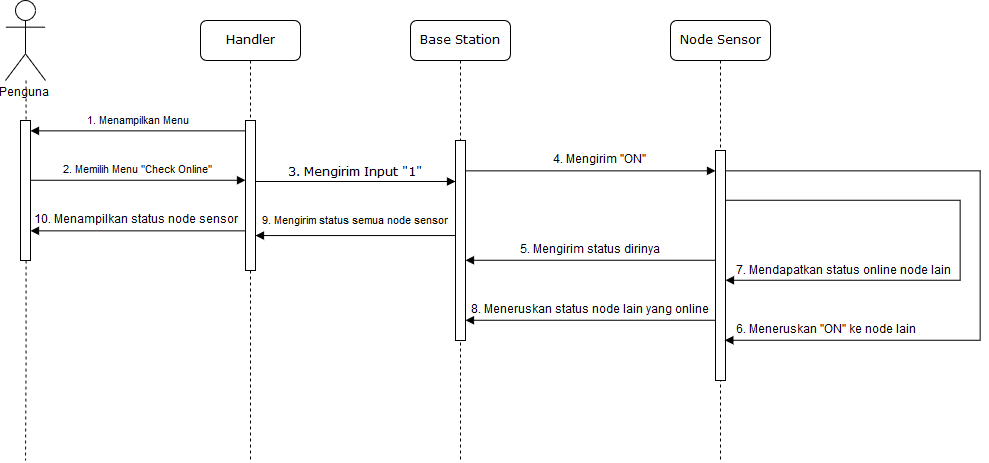
\includegraphics[scale=0.5]{sequenceOnline}
	\caption{Diagram Sequence "Check Online"}
	\label{fig:sequenceOnline}
\end{figure}
Fitur ini diawali dengan Handler sebagai program komputer pengguna menampilkan pilihan yang dapat dipilih oleh pengguna. Kemudian pengguna memilih "Check Online". "Check Online" ini digunakan untuk mengetahui node sensor yang sedang menyala (\textit{online}). Handler mengirimkan input "1" kepada \textit{base station}. Lalu \textit{base station} mengirimkan "ON" kepada node sensor. Saat node sensor mendapatkan pesan "ON", node sensor akan mengirimkan status dirinya dan meneruskan pesan "ON" kepada node sensor lain. Node sensor juga mendapatkan status dari node sensor lain dan diteruskan hingga sampai ke \textit{base station}. Kemudian \textit{base station} mendapatkan status dari semua node sensor dan meneruskan Handler. Handler yang akan menampilkan status node sensor kepada pengguna.
\subsection{Diagram Sequence "Synchronize Time"}
\begin{figure}[H]
	\centering
	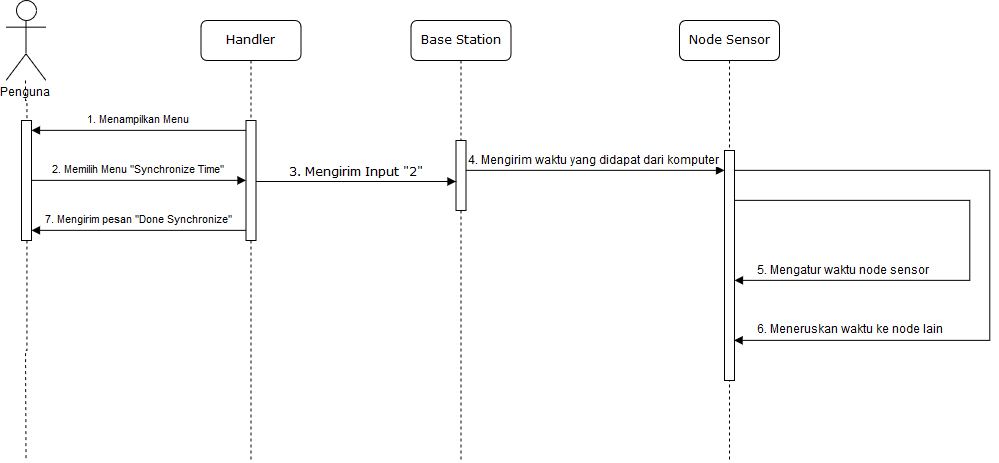
\includegraphics[scale=0.5]{sequenceSynchronize}
	\caption{Diagram Sequence "Synchronize Time"}
	\label{fig:sequenceSynchronize}
\end{figure}
Fitur ini diawali dengan Handler menampilkan pilihan yang dapat dipilih oleh pengguna. Kemudian pengguna memilih "Synchronize Time". "Synchronize Time" ini digunakan untuk melakukan sinkronisasi waktu semua node sensor sesuai dengan waktu lokal pada komputer pengguna. Saat pertama menjalankan program, \textit{base station} mengatur waktu sesuai waktu komputer pengguna. Handler mengirimkan input "2" kepada \textit{base station}. Kemudian \textit{base station} meneruskan waktu kepada node sensor dan node sensor ini meneruskan waktu kepada node sensor lain. Setelah pengguna memilih "Synchronize Time", Handler akan mengirimkan pesan "Done Synchronize".

\subsection{Diagram Sequence "Get Time"}
\begin{figure}[H]
	\centering
	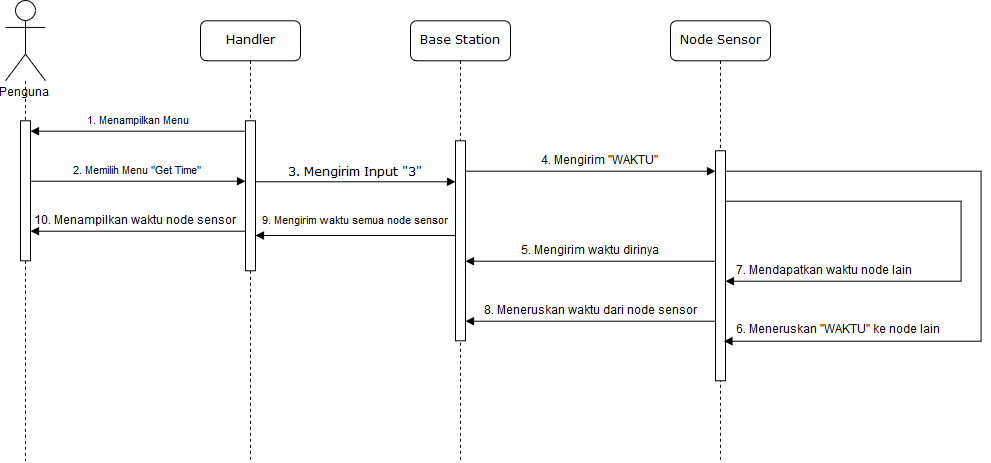
\includegraphics[scale=0.5]{sequenceGetTime}
	\caption{Diagram Sequence "Get Time"}
	\label{fig:sequenceGetTime}
\end{figure}
Fitur ini diawali dengan Handler menampilkan pilihan yang dapat dipilih oleh pengguna. Kemudian pengguna memilih "Get Time". "Get Time" ini digunakan untuk mendapatkan waktu dari setiap node sensor. Handler mengirimkan input "3" kepada \textit{base station}. Kemudian \textit{base station} mengirimkan pesan "WAKTU" kepada node sensor dan node sensor meneruskan pesan "WAKTU" kepada node sensor tetangganya. Setelah itu node sensor akan mengirimkan waktu kepada \textit{base station} atau node sensor lain. \textit{Base station} mengirimkan waktu node sensor kepada Handler dan Handler yang akan menampilkan kepada pengguna.

\subsection{Diagram Sequence "Start Sensing"}
\begin{figure}[H]
	\centering
	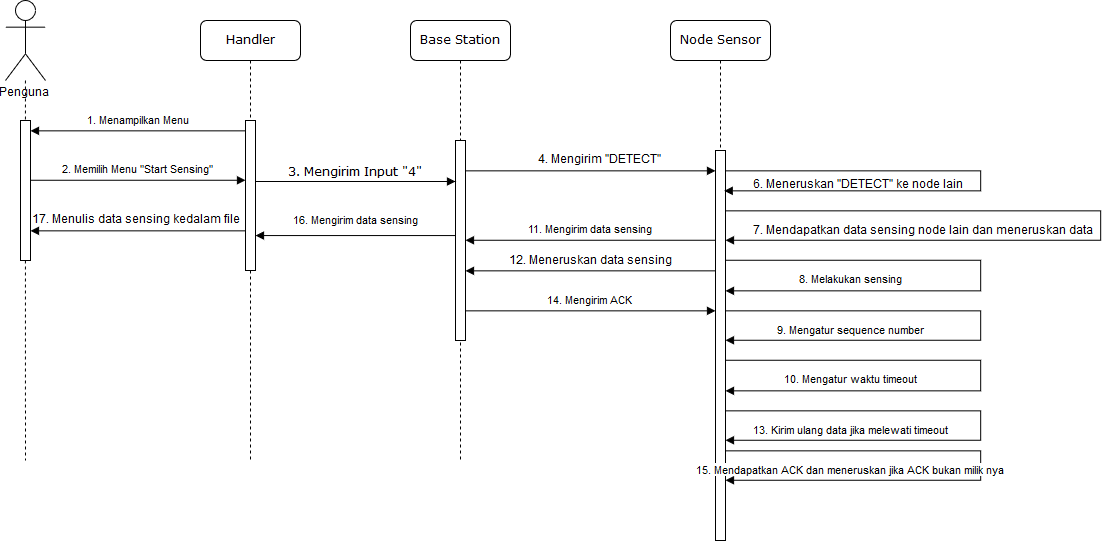
\includegraphics[scale=0.45]{sequenceSensing}
	\caption{Diagram Sequence "Start Sensing"}
	\label{fig:sequenceSensing}
\end{figure}
Fitur ini digunakan untuk mendapatkan data sensing secara \textit{reliable}. Setelah Handler menampilkan pilihan untuk dipilih pengguna dan pengguna memilih untuk memulai \textit{sensing}, Handler meneruskan pilihan tersebut kepada \textit{base station}. \textit{Base station} mengirimkan pesan "DETECT" kepada node sensor. Node sensor melakukan \textit{sensing}, mengatur \textit{sequence number}, dan mengatur \textit{timeout}. Kemudian node sensor meneruskan pesan "DETECT" kepada node sensor lain. Setelah melakukan \textit{sensing}, node sensor akan mengirimkan data kepada node sensor lain atau langsung kepada \textit{base station}. Jika data hasil \textit{sensing} dikirim kepada node sensor lain, maka data tersebut akan diteruskan hingga sampai ke \textit{base station}. Data yang sudah sampai \textit{base station} akan diteruskan kepada Handler untuk ditulis ke dalam \textit{file} agar dapat dibaca oleh pengguna. 

\subsection{Diagram Sequence "Exit"}
\begin{figure}[H]
	\centering
	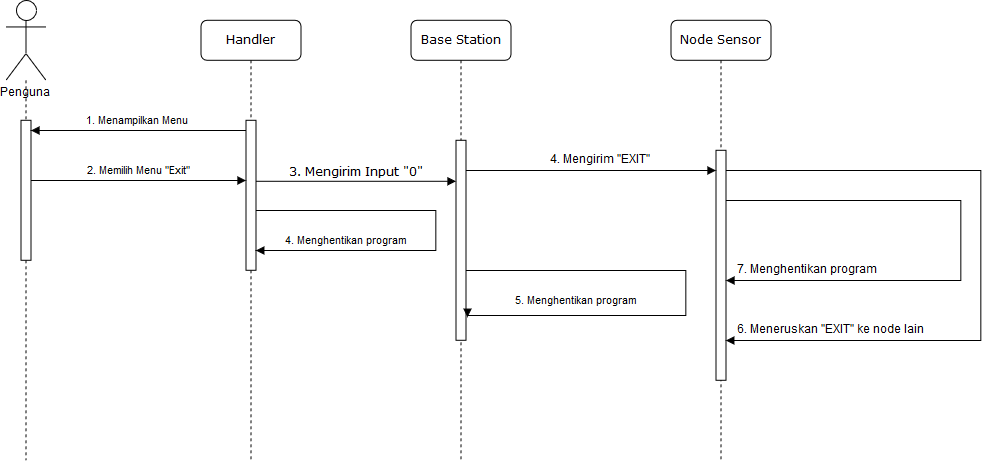
\includegraphics[scale=0.5]{sequenceExit}
	\caption{Diagram Sequence "Exit"}
	\label{fig:sequenceExit}
\end{figure}
Fitur ini digunakan untuk menghentikan semua proses yang sedang berlangsung pada Handler, \textit{Base Station}, dan Node Sensor. Fitur ini diawali dengan Handler menampilkan pilihan yang dapat dipilih oleh pengguna. Kemudian pengguna memilih "Exit". Handler mengirimkan input "0" yang berarti \textit{exit} kepada \textit{base station} dan menghentikan program yang sedang berjalan. \textit{Base station} mengirimkan pesan "EXIT" kepada node sensor lain dan menghentikan program pada \textit{base station}. Node sensor yang menerima pesan "EXIT" juga menghentikan program yang sedang berjalan.

\section{Perancangan Kelas Aplikasi Transfer Data Di WSN}
Pada subbab \ref{subsec:fitur_dan_kebutuhan_sistem} telah dijelaskan kelas diagram aplikasi transfer data secara sederhana. Pada subbab ini dijelaskan kelas diagram secara detail dengan Gambar~\ref{fig:sensor} sampai Gambar~\ref{fig:handler}. Deskripsi setiap kelas dijelaskan sebagai berikut:
\begin{itemize}
    \item \textbf{Package Sensor}
    \begin{figure}[h]
    	\centering
    	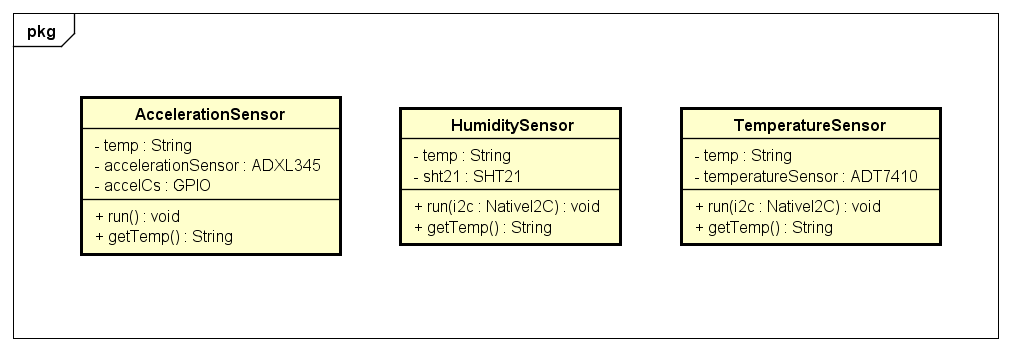
\includegraphics[scale=0.65]{sensor}
    	\caption{Diagram Kelas Sensor-Sensor}
    	\label{fig:sensor}
    \end{figure}
    \begin{itemize}
        \item \textbf{Kelas AccelerationSensor}\\
        Kelas ini digunakan untuk melakukan pengukuran tekanan udara pada satu waktu. Atribut-atribut pada kelas ini adalah sebagai berikut:
        \begin{itemize}
            \item private ADXL345 accelerationSensor\\
            Atribut ini digunakan sebagai \textit{import} dari \textit{driver sensor} untuk mengukur getaran yang ada pada node sensor Preon32.
            \item private String temp\\
            Atribut ini digunakan untuk menyimpan sementara data hasil pengukuran tekanan udara pada satu waktu.
            \item private GPIO accelSc\\
            Atribut ini digunakan sebagai \textit{import} dari \textit{driver GPIO} (general purpose IO).
        \end{itemize}
        Metode-metode pada kelas ini adalah sebagai berikut:
        \begin{itemize}
            \item public void run()\\
            Metode ini digunakan untuk melakukan \textit{sensing} getaran dan datanya akan disimpan pada atribut temp.
            \item public String getTemp()\\
            Metode ini digunakan untuk mengembalikan atribut temp yang nanti digunakan pada kelas-kelas lain.
        \end{itemize}
        \item \textbf{Kelas HumiditySensor}\\
        Kelas ini digunakan untuk melakukan pengukuran kelembaban pada satu waktu. Atribut-atribut pada kelas ini adalah sebagai berikut:
        \begin{itemize}
            \item private SHT21 sht21\\
            Atribut ini digunakan sebagai \textit{import} dari \textit{driver sensor} untuk mengukur kelembaban yang ada pada node sensor Preon32.
            \item private String temp\\
            Atribut ini digunakan untuk menyimpan sementara data hasil pengukuran kelembaban pada satu waktu.
        \end{itemize}
        Metode-metode pada kelas ini adalah sebagai berikut:
        \begin{itemize}
            \item public void run(NativeI2C i2c)\\
            Metode ini digunakan untuk melakukan \textit{sensing} kelembaban dan datanya akan disimpan pada atribut temp.
            \item public String getTemp()\\
            Metode ini digunakan untuk mengembalikan atribut temp yang nanti digunakan pada kelas-kelas lain.
        \end{itemize}
        \item \textbf{Kelas TemperatureSensor}\\
        Kelas ini digunakan untuk melakukan pengukuran suhu pada satu waktu. Atribut-atribut pada kelas ini adalah sebagai berikut:
        \begin{itemize}
            \item private ADT7410 temperatureSensor\\
            Atribut ini digunakan sebagai \textit{import} dari \textit{driver sensor} untuk mengukur suhu yang ada pada node sensor Preon32.
            \item private String temp\\
            Atribut ini digunakan untuk menyimpan sementara data hasil pengukuran suhu pada satu waktu.
        \end{itemize}
        Metode-metode pada kelas ini adalah sebagai berikut:
        \begin{itemize}
            \item public void run(NativeI2C i2c)\\
            Metode ini digunakan untuk melakukan \textit{sensing} suhu dan datanya akan disimpan pada atribut temp.
            \item public String getTemp()\\
            Metode ini digunakan untuk mengembalikan atribut temp yang nanti digunakan pada kelas-kelas lain.
        \end{itemize}
    \end{itemize}
    \item \textbf{Package main}
    \begin{itemize}
        \item \textbf{Kelas Sensing}\\
        \begin{figure}[h]
        	\centering
        	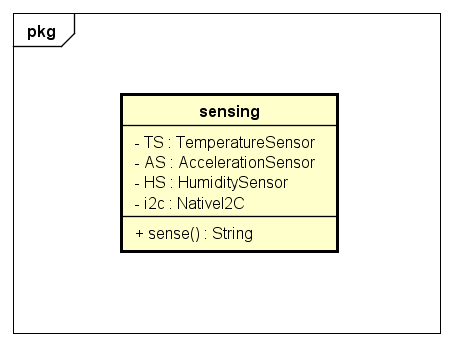
\includegraphics[scale=1]{sensing}
        	\caption{Diagram Kelas Sensing}
        	\label{fig:sensing}
        \end{figure}
        Kelas ini menyatukan tiga buah kelas sensor dan digunakan pada kelas NS. Atribut-atribut pada kelas ini adalah sebagai berikut:
        \begin{itemize}
            \item private TemperatureSensor TS = new TemperatureSensor()\\
            Atribut untuk membuat objek baru dari kelas TemperatureSensor.
            \item private AccelerationSensor AS = new AccelerationSensor()\\
            Atribut untuk membuat objek baru dari kelas AccelerationSensor.
            \item private HumiditySensor HS = new HumiditySensor()\\
            Atribut untuk membuat objek baru dari kelas HumiditySensor.
            \item private NativeI2C i2c = NativeI2C.getInstance(1)\\
            Atribut untuk melakukan inisialisasi \textit{driver NativeI2C} untuk digunakan oleh sensor-sensor.
        \end{itemize}
        Metode-metode pada kelas ini adalah sebagai berikut:
        \begin{itemize}
            \item public String sense()\\
            Metode ini digunakan untuk melakukan \textit{sensing}. Metode ini mengembalikan \textit{string} yang berisi nilai \textit{sensing} dari setiap sensor yang digunakan.
        \end{itemize}
        \item \textbf{Kelas BS}\\
        \begin{figure}[h]
        	\centering
        	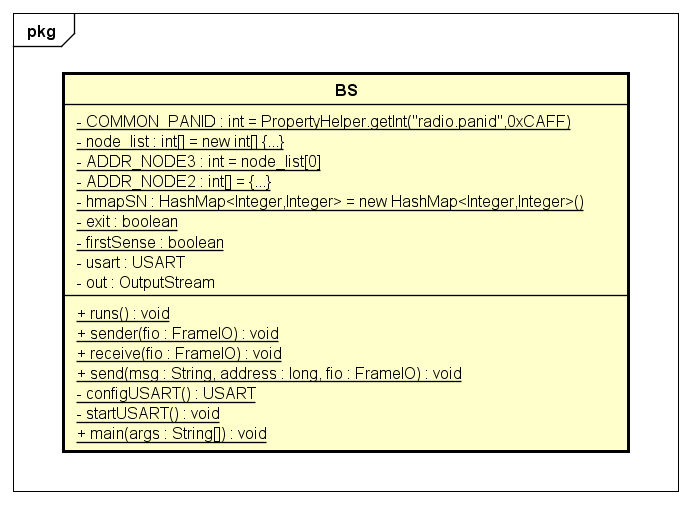
\includegraphics[scale=0.7]{basestation}
        	\caption{Diagram Kelas BS}
        	\label{fig:basestation}
        \end{figure}
        Kelas ini menangani fungsi-fungsi yang ada pada \textit{base station} seperti mengirimkan perintah-perintah kepada node sensor dibawahnya dan menerima data dari node sensor. Kelas ini yang akan diunggah kedalam node sensor \textit{base station}. Atribut-atribut pada kelas ini adalah sebagai berikut:
        \begin{itemize}
            \item private static int COMMON\_PANID\\
            Atribut ini digunakan untuk menyimpan PAN ID dari satu jaringan node sensor.
            \item private static int [] node\_list\\
            Atribut ini digunakan untuk menyimpan daftar alamat node sensor pada satu jaringan.
            \item private static int ADDR\_NODE3\\
            Atribut ini digunakan untuk menyimpan alamat dari \textit{base station}.
            \item private static int[] ADDR\_NODE2\\
            Atribut ini menyimpan alamat node sensor yang terhubung langsung \textit{base station}.
            \item private static HashMap<Long, Integer> hmap\\
            Atribut ini digunakan untuk menyimpan sementara data dari setiap node sensor yang ada pada node\_list untuk memastikan \textit{reliability}.
            \item private static boolean exit\\
            Atribut ini digunakan menyimpan kondisi exit saat mendapatkan input "Exit" dari user.
            \item private static boolean firstSense\\
            Atribut ini digunakan untuk menyimpan kondisi sudah melakukan \textit{sensing} atau belum.
            \item private static USART usart\\
            Atribut ini digunakan untuk inisialisasi USART yang menghubungkan \textit{base station} dengan komputer yang terhubung langsung.
            \item private static OutputStream out\\
            Atribut ini digunakan untuk inisialisasi OutputStream yang menulis data dari \textit{base station} ke program komputer agar bisa dilihat oleh pengguna.
        \end{itemize}
        Metode-metode pada kelas ini adalah sebagai berikut:
        \begin{itemize}
            \item public void runs()\\
            Metode ini digunakan untuk memanggil metode sender().
            \item public static void sender(Final FrameIO fio)\\
            Metode ini digunakan untuk melakukan mengirim perintah-perintah ke node sensor.
            \item public static void receiver(Final FrameIO fio)\\
            Metode ini digunakan untuk menerima data dari node sensor. 
            \item public void send(String msg, long address, FrameIO fio)\\
            Metode ini digunakan untuk mengirimkan pesan (\textit{msg}) dari \textit{base station} ke alamat tujuan (\textit{address}) dengan menggunakan FrameIO (\textit{fio}).
            \item public static void main(String[] args)\\
            Metode ini digunakan sebagai metode utama dari kelas ini dan memanggil metode runs().
        \end{itemize}
        \item \textbf{Kelas NS}\\
        \begin{figure}[htbp]
        	\centering
        	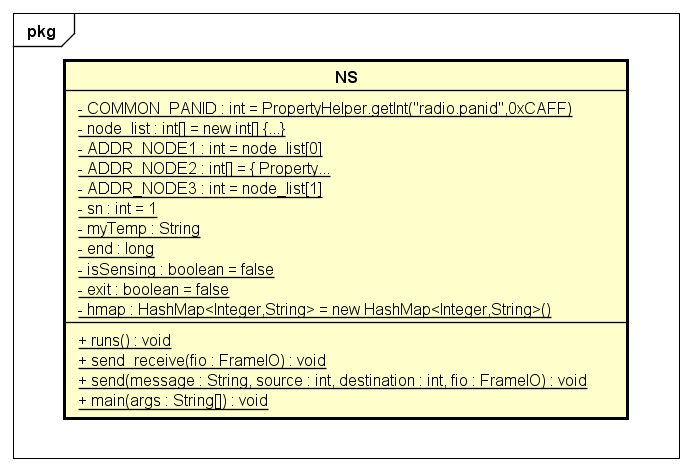
\includegraphics[scale=0.7]{nodesensor}
        	\caption{Diagram Kelas NS}
        	\label{fig:nodesensor}
        \end{figure}
        Kelas ini diunggah ke dalam node sensor untuk melakukan \textit{sensing} dan mengirimkan data ke \textit{base station} atau ke node sensor lain. Atribut-atribut pada kelas ini adalah sebagai berikut:
        \begin{itemize}
            \item private static int COMMON\_PANID\\
            Atribut ini digunakan untuk menyimpan PAN ID dari satu jaringan node sensor.
            \item private static int [] node\_list\\
            Atribut ini digunakan untuk menyimpan daftar alamat node sensor pada satu jaringan.
            \item private int ADDR\_NODE1\\
            Atribut ini digunakan untuk menyimpan alamat dari node sensor diatas node sensor ini.
            \item private static int[] ADDR\_NODE2\\
            Atribut ini menyimpan array alamat yang terhubung langsung node sensor ini kecuali node \textit{base station}.
            \item private static int ADDR\_NODE3\\
            Atribut ini digunakan untuk menyimpan alamat dari node sensor ini.
            \item private sensing s\\
            Atribut ini digunakan untuk membuat objek dari kelas Sensing.
            \item private int sn = 1\\
            Atribut ini digunakan untuk menyimpan \textit{counter} dari \textit{sequence number} pada satu kali pengiriman \textit{frame}.
            \item private static String myTemp\\
            Atribut ini digunakan untuk menyimpan sementara data hasil sensing dari node sensor ini.
            \item private static long end\\
            Atribut ini digunakan untuk menyimpan batas waktu node sensor menunggu ACK / NACK (\textit{timeout}).
            \item private static boolean isSensing\\
            Atribut ini digunakan sebagai penanda bahwa sudah pernah melakukan sensing agar tidak melakukan sensing lagi sebelum menerima ACK.
            \item private static boolean exit\\
            Atribut ini digunakan sebagai penanda program telah dihentikan dari \textit{base station} dah harus dihentikan juga pada node sensor ini.
            \item private static HashMap<Integer, String> hmap\\
            Atribut ini digunakan untuk menyimpan sementara data sensing dari node tetangga pada atribut ADDR\_NODE2. untuk memastikan reliability sampai ke \textit{base station}.
        \end{itemize}
        Metode-metode pada kelas ini adalah sebagai berikut:
        \begin{itemize}
            \item public void runs()\\
            Metode ini berisi inisialisai dari radio, transmiter dan memanggil method send\_receive().
            \item public void send\_receive(Final FrameIO fio)\\
            Metode ini digunakan node sensor untuk menangani pengiriman dan penerimaan data.
            \item public void send(String message, int source, int destination, FrameIO fio)\\
            Metode ini digunakan untuk mengirim pesan (\textit{message}) dari dirinya (\textit{source}) kepada tujuan (\textit{destination} dengan FrameIO (\textit{fio}).
            \item public static void main(String[] args)\\
            Metode ini digunakan sebagai metode utama dari kelas ini dan memanggil metode runs().
        \end{itemize}
        \item \textbf{Kelas BS\_Testing}\\
        \begin{figure}[h]
        	\centering
        	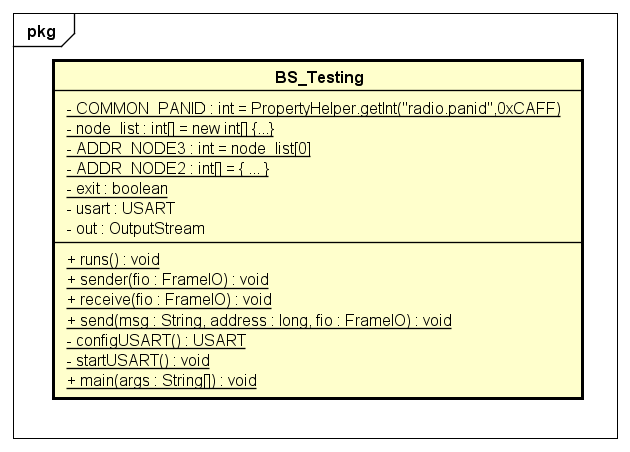
\includegraphics[scale=0.7]{bs_testing}
        	\caption{Diagram Kelas BS\_Testing}
        	\label{fig:bs_testing}
        \end{figure}
        Kelas ini menangani fungsi-fungsi yang ada pada \textit{base station} seperti mengirimkan perintah-perintah kepada node sensor dibawahnya dan menerima data dari node sensor. Kelas ini yang akan diunggah kedalam node sensor \textit{base station}. Kelas ini digunakan sebagai \textit{base station} yang tidak menangani \textit{reliability}. Atribut-atribut pada kelas ini adalah sebagai berikut:
        \begin{itemize}
            \item private static int COMMON\_PANID\\
            Atribut ini digunakan untuk menyimpan PAN ID dari satu jaringan node sensor.
            \item private static int [] node\_list\\
            Atribut ini digunakan untuk menyimpan daftar alamat node sensor pada satu jaringan.
            \item private static int ADDR\_NODE3\\
            Atribut ini digunakan untuk menyimpan alamat dari \textit{base station}.
            \item private static int[] ADDR\_NODE2\\
            Atribut ini menyimpan alamat node sensor yang terhubung langsung \textit{base station}.
            \item private static boolean exit\\
            Atribut ini digunakan menyimpan kondisi exit saat mendapatkan input "Exit" dari user.
            \item private static USART usart\\
            Atribut ini digunakan untuk inisialisasi USART yang mengubungkan \textit{base station} dengan komputer yang terhubung langsung.
            \item private static OutputStream out\\
            Atribut ini digunakan untuk inisialisasi OutputStream yang menulis data dari node sensor ke program komputer agar bisa dilihat oleh pengguna.
        \end{itemize}
        Metode-metode pada kelas ini adalah sebagai berikut:
        \begin{itemize}
            \item public void runs()\\
            Metode ini digunakan untuk memanggil metode sender() dan receiver().
            \item public static void sender(Final FrameIO fio)\\
            Metode ini digunakan untuk melakukan mengirim perintah-perintah ke node sensor.
            \item public static void receiver(Final FrameIO fio)\\
            Metode ini digunakan untuk menerima data dari node sensor. 
            \item public void send(String msg, long address, FrameIO fio)\\
            Metode ini digunakan untuk mengirimkan pesan (\textit{msg}) dari \textit{base station} ke alamat tujuan (\textit{address}) dengan menggunakan FrameIO (\textit{fio}).
            \item public static void main(String[] args)\\
            Metode ini digunakan sebagai metode utama dari kelas ini dan memanggil metode runs().
        \end{itemize}
        \item \textbf{Kelas NS\_Testing}\\
        \begin{figure}[htbp]
        	\centering
        	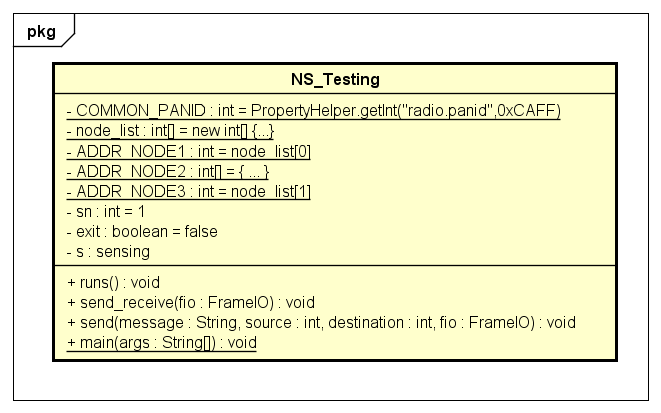
\includegraphics[scale=0.65]{ns_testing}
        	\caption{Diagram Kelas NS\_Testing}
        	\label{fig:ns_testing}
        \end{figure}
        Kelas ini diunggah ke dalam node sensor untuk melakukan \textit{sensing} dan mengirimkan data ke \textit{base station} atau ke node sensor lain. Kelas ini digunakan sebagai node sensor yang tidak menangani \textit{reliability}. Atribut-atribut pada kelas ini adalah sebagai berikut:
        \begin{itemize}
            \item private static int COMMON\_PANID\\
            Atribut ini digunakan untuk menyimpan PAN ID dari satu jaringan node sensor.
            \item private static int [] node\_list\\
            Atribut ini digunakan untuk menyimpan daftar alamat node sensor pada satu jaringan.
            \item private int ADDR\_NODE1\\
            Atribut ini digunakan untuk menyimpan alamat dari node sensor diatas node sensor ini.
            \item private static int[] ADDR\_NODE2\\
            Atribut ini menyimpan array alamat yang terhubung langsung node sensor ini kecuali node \textit{base station}.
            \item private static int ADDR\_NODE3\\
            Atribut ini digunakan untuk menyimpan alamat dari node sensor ini.
            \item private sensing s\\
            Atribut ini digunakan untuk membuat objek dari kelas Sensing.
            \item private int sn = 1\\
            Atribut ini digunakan untuk menyimpan \textit{counter} dari \textit{sequence number} pada satu kali pengiriman \textit{frame}.
            \item private boolean exit\\
            Atribut ini digunakan sebagai penanda program telah dihentikan dari \textit{base station} dah harus dihentikan juga pada node sensor ini.
        \end{itemize}
        Metode-metode pada kelas ini adalah sebagai berikut:
        \begin{itemize}
            \item public void runs()\\
            Metode ini berisi inisialisai dari radio, transmiter dan memanggil method send\_receive().
            \item public void send\_receive(Final FrameIO fio)\\
            Metode ini digunakan node sensor untuk menangani pengiriman dan penerimaan data.
            \item public void send(String message, int source, int destination, FrameIO fio)\\
            Metode ini digunakan untuk mengirim pesan (\textit{message}) dari dirinya (\textit{source}) kepada tujuan (\textit{destination} dengan FrameIO (\textit{fio}).
            \item public static void main(String[] args)\\
            Metode ini digunakan sebagai metode utama dari kelas ini dan memanggil metode runs().
        \end{itemize}
    \end{itemize}
    \item \textbf{Package Handler}
    \begin{itemize}
        \item \textbf{Kelas Handler}\\
        \begin{figure}[h]
        	\centering
        	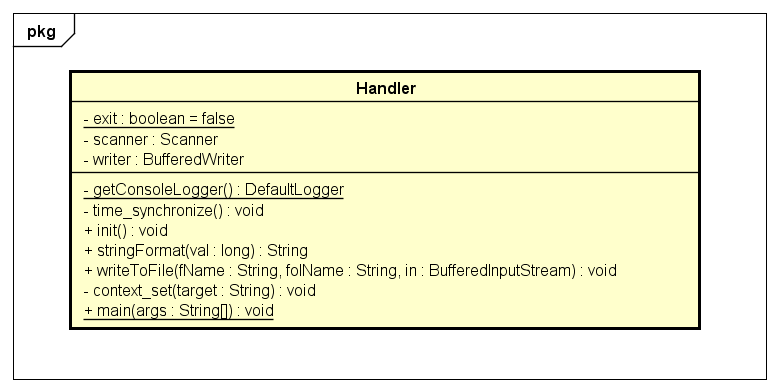
\includegraphics[scale=0.7]{handler}
        	\caption{Diagram Kelas Handler}
        	\label{fig:handler}
        \end{figure}
        Kelas ini menangani hubungan antara \textit{base station} dengan komputer pengguna. Saat menerima data, \textit{base station} akan mengirimkan data yang diterima kepada kelas Handler. Kelas Handler ini akan mengelola data yang diterima dan ditampilkan atau ditulis kedalam file.
        Atribut-atribut pada kelas ini adalah sebagai berikut:
        \begin{itemize}
            \item private volatile static boolean exit = false\\
            Atribut ini digunakan untuk \textit{variable} exit. Saat pengguna memasukan angka 0, maka exit akan menjadi \textit{true}, dan program akan berhenti.
            \item private Scanner scanner\\
            Atribut ini digunakan untuk inisialisasi Scanner sebagai masukan pengguna pada CLI.
            \item private BufferedWriter writer\\
            Atribut ini digunakan untuk membuat objek BufferedWriter yang digunakan untuk menulis data \textit{sensing} kedalam file.
        \end{itemize}
        Metode-metode pada kelas ini adalah sebagai berikut:
        \begin{itemize}
            \item private static DefaultLogger getConsoleLogger()\\
            Metode ini digunakan untuk memunculkan tulisan pada \textit{console}.
            \item private void time\_synchronize()\\
            Metode ini digunakan untuk melakukan sinkronisasi waktu \textit{base station} sesuai dengan waktu pada komputer saat itu.
            \item public void init()\\
            Metode ini digunakan untuk membangun koneksi antara program pada komputer dengan program pada \textit{base station}. Pada metode ini juga terdapat pilihan yang dapat dipilih pengguna dan mengirimkan masukan tersebut kepada \textit{base station}.
            \item public String stringFormat(long val)\\
            Metode ini digunakan untuk mengubah format dari waktu yang didapat dari node sensor sehingga dapat dibaca oleh pengguna.
            \item public void writeToFile(String fName, String folName, BufferedInputStream in)\\
            Metode ini digunakan untuk menulis data sensing kedalam file.
            \item private void context\_set(String target)\\
            Metode ini digunakan untuk memilih \textit{context} yang akan digunakan.
            \item public static void main(String[] args)\\
            Metode ini digunakan sebagai metode utama untuk menjalankan kelas ini. Metode ini memanggil metode context\_set(), time\_synchronize(), dan init().
        \end{itemize}
    \end{itemize}
\end{itemize}

\section{Perancangan Masukan dan Keluaran}
Aplikasi transfer data yang dibangun menggunakan \textit{command line interface} sebagai media penerima masukan dan mengeluarkan keluaran. Aplikasi ini dapat menerima masukan dengan tipe \textit{integer}. Akan tersedia 5 buah pilihan, pengguna dapat memasukkan nilai 1-4 dan 0 sebagai masukan. Masukan yang diberikan oleh pengguna antara lain adalah :
\begin{itemize}
\item \textbf{Masukan dengan nilai 1} digunakan untuk mengetahui node mana saja yang sedang menyala. Keluaran dari masukan ini adalah nama node diikuti dengan status \textit{online}.
\item \textbf{Masukan dengan nilai 2} digunakan untuk melakukan sinkronisasi waktu setiap node sensor sesuai dengan node waktu pada \textit{base station}. Keluaran dari masukan ini adalah pesan berhasil melakukan sinkronisasi waktu.
\item \textbf{Masukan dengan nilai 3} digunakan untuk mendapatkan waktu dari setiap node sensor. Keluaran dari masukan ini adalah nama node sensor diikuti dengan waktu pada node sensor tersebut.
\item \textbf{Masukan dengan nilai 4} digunakan untuk memulai \textit{sensing} dari setiap node sensor. Keluaran dari masukan ini adalah pesan mulai melakukan \textit{sensing} dan setiap data hasil sensing tersebut ditulis kedalam file text.
\item \textbf{Masukan dengan nilai 0} digunakan untuk menghentikan dan keluar dari aplikasi. Saat pengguna memasukkan nilai 0, sistem memperlihatkan pesan keluar dari aplikasi dan berhenti menerima masukan dari pengguna.
\item Apabila pengguna memasukkan nilai \textbf{masukan yang tidak valid}, sistem akan memberikan keluaran pesan bahwa pesan tidak \textit{valid} serta menampilkan kembali pilihan. 
\end{itemize} 

\section{Perancangan Pseudocode Aplikasi Transfer Data Yang Reliable}
Pada subbab ini dirancang \textit{pseudocode} untuk membuat aplikasi transfer data yang \textit{reliable}. \textit{Pseudocode} yang dibuat digunakan pada program \textit{base station} dan \textit{node sensor} terkait dengan pengiriman pesan atau data hasil \textit{sensing}.

\subsection{Base Station}
Untuk melakukan pengiriman dan penerimaan pesan, \textit{base station} menggunakan 2 metode yang terpisah. Metode sender digunakan untuk mengirim perintah kepada node sensor. Sedangkan metode receiver digunakan untuk menerima data dari node sensor.
\begin{algorithm}[htbp]
\caption{Metode sender}
\begin{algorithmic}[1]
\Function{sender}{}
    \State \textbf{thread} $\leftarrow$ thread baru \textbf{do}
        \Indent
            \Function{run}{}
                \While{true}
                    \State temp $\leftarrow$ membuat variable lokal
                        \try
                            \State temp $\leftarrow$ usart.read() // membaca masukan dari pengguna
                        \catch{USARTException}
                        \endtry
                        \If{temp = 0}
                            \State mengirim pesan "EXIT" kepada semua node ADDR\_NODE2
                        \ElsIf{temp = 1}
                            \State mengirim pesan "ON" kepada semua node ADDR\_NODE2
                        \ElsIf{temp = 2}
                            \State mengirim pesan "("Q" + currTime)" kepada semua node ADDR\_NODE2
                        \ElsIf{temp = 3}
                            \State mengirim pesan "WAKTU" kepada semua node ADDR\_NODE2
                        \ElsIf{temp = 4}
                            \State mengirim pesan "DETECT" kepada semua node ADDR\_NODE2
                        \EndIf
                \EndWhile
            \EndFunction
        \EndIndent
    \State \textbf{end thread}
    \State thread.start()
\EndFunction
\end{algorithmic}
\end{algorithm}

\begin{algorithm}[htbp]
\caption{Metode receive}
\begin{algorithmic}[1]
\Function{receive}{}
    \State \textbf{thread} receive $\leftarrow$ thread baru \textbf{do}
        \Indent
            \Function{run}{}
                \State frame $\leftarrow$ membuat objek frame baru
                \While{true}
                    \try
                        \State fio.receive(frame) // menerima frame
                        \State dg $\leftarrow$ mendapatkan isi dari payload sebuah frame
                        \State str $\leftarrow$ mengubah dg menjadi string
                        \If{str.charAt(str.length()-1) = 'E'}
                            \State merupakan pesan status menyala dari node sensor
                            \try
                                \State menulis pesan agar dapat dibaca pengguna
                                \State out.write(msg.getBytes(), 0, msg.length())
                                \State usart.flush()
                            \catch{Exception}
                            \endtry
                        \ElsIf{str.charAt(0) = 'T'}
                            \State merupakan pesan waktu node sensor
                            \try
                                \State menulis pesan agar dapat dibaca pengguna
                                \State out.write(msg.getBytes(), 0, msg.length())
                                \State usart.flush()
                            \catch{Exception}
                            \endtry
                        \ElsIf{str.startsWith("SENSE")}
                            \State merupakan pesan data hasil sensing dari node sensor
                            \State node $\leftarrow$ alamat node sensor yang mengirim data
                            \State sn $\leftarrow$ sequence number dari data yang diterima
                            \If{hmapSN.get(node)=sn}
                                \State apakah sequence number data yang diterima sesuai urutan 
                                \try
                                    \State menulis pesan agar dapat dibaca pengguna
                                    \State out.write(msg.getBytes(), 0, msg.length()) 
                                    \State usart.flush()
                                \catch{Exception}
                                \endtry
                                \State hmapSN.put(node, sn+1)
                            \EndIf
                            \State base station akan mengirimkan ACK setiap kali menerima data hasil sensing
                        \EndIf
                    \catch{Exception}
                    \endtry
                \EndWhile
            \EndFunction
        \EndIndent
    \State \textbf{end thread}
    \State receive.start()
\EndFunction
\end{algorithmic}
\end{algorithm}

\subsection{Node Sensor}
Berbeda dengan \textit{base station}, node sensor hanya menggunakan 1 metode untuk menangani pengiriman dan penerimaan pesan yaitu metode send\_receive.
\begin{algorithm}[htbp]
\caption{Metode send\_receive}
\begin{algorithmic}[1]
\Function{send\_receive}{}
    \State \textbf{thread} thread $\leftarrow$ thread baru \textbf{do}
        \Indent
            \Function{run}{}
                \State frame $\leftarrow$ membuat objek frame baru
                \While{true}
                    \try
                        \State fio.receive(frame) // menerima frame
                        \State dg $\leftarrow$ mendapatkan payload dari frame
                        \State str $\leftarrow$ mengubah dg menjadi string
                        \If{str.charAt(0) == 'Q'}
                            \State merupakan pesan dari base station untuk sinkronisasi waktu
                            \State Time.setCurrentTimeMillis(currTime)
                            \If{ADDR\_NODE2.length > 0}
                                \State meneruskan waktu base station kepada semua node ADDR\_NODE2
                            \EndIf
                        \ElsIf{str.charAt(0) = 'T'}
                            \State merupakan pesan berisi waktu dari node ADDR\_NODE2
                            \State pesan diteruskan kepada node ADDR\_NODE1
                        \ElsIf{str.equalsIgnoreCase("EXIT")}
                            \State merupakan pesan untuk menghentikan program dari base station
                            \State isSensing $\leftarrow$ false
                            \State exit $\leftarrow$ true
                            \If{ADDR\_NODE2.length > 0}
                                \State meneruskan pesan "EXIT" kepada semua node ADDR\_NODE2
                            \EndIf
                        \ElsIf{str.equalsIgnoreCase("WAKTU")}
                            \State merupakan pesan untuk meminta waktu dari setiap node sensor
                            \State msg $\leftarrow$ "Time "ADDR\_NODE3 +" " + Time.currentTimeMillis()
                            \State node sensor mengirimkan msg kepada ADDR\_NODE1
                            \If{ADDR\_NODE2.length > 0}
                                \State meneruskan pesan "WAKTU" kepada semua node ADDR\_NODE2
                            \EndIf
                        \ElsIf{str.equalsIgnoreCase("ON")}
                            \State merupakan pesan untuk meminta status menyala dari setiap node sensor
                            \State msg $\leftarrow$ pesan bahwa node tersebut online
                            \State mengirim msg kepada node ADDR\_NODE1
                            \If{ADDR\_NODE2.length > 0}
                                \State meneruskan pesan "ON" kepada semua node ADDR\_NODE2
                            \EndIf
\algstore{myalg}
\end{algorithmic}
\end{algorithm}

\begin{algorithm}[H]
\begin{algorithmic}
\algrestore{myalg}
                        \ElsIf{str.charAt(str.length()$-$1) = 'E'}
                            \State meneruskan status menyala dari node sensor lain kepada ADDR\_NODE1.
                    \ElsIf{str.equalsIgnoreCase("DETECT")}
                            \State menerima perintah melakukan sensing.
                            \State message $\leftarrow$ membuat format pesan pengiriman data hasil sensing
							\State myTemp $\leftarrow$ message
							\State sn++
							\If{ADDR\_NODE2.length > 0}
                                \State meneruskan pesan "DETECT" kepada semua node ADDR\_NODE2
                            \EndIf
                            \State mengirim myTemp kepada ADDR\_NODE1
                            \State end $\leftarrow$ mengatur timer batas menunggu ACK
                            \State isSensing $\leftarrow$ true
                        \ElsIf{str.charAt(0) = 'S'}
                            \State mendapatkan data hasil sensing dari node sensor lain
                            \State meneruskan data hasil sensing kepada node ADDR\_NODE1
                        \ElsIf{str.startWith("ACK")}
                            \State menerima ACK
                            \State node $\leftarrow$ node yang ada pada pesan ACK
                            \If{node = ADDR\_NODE3}
                                \State se $\leftarrow$ sequence number pada pesan ACK
                                \If{se = sn$-$1}
                                    \State isSensing $\leftarrow$ false
                                    \State message $\leftarrow$ melakukan sensing dan membuat format pesan data sensing
									\State myTemp $\leftarrow$ message
									\State sn++
									\State mengirim data sensing kepada node ADDR\_NODE1
									\State end $\leftarrow$ mengatur timer batas menunggu ACK
									\State isSensing $\leftarrow$ true
                                \Else
                                    \State mengirim myTemp kepada ADDR\_NODE1
                                    \State end $\leftarrow$ mengatur timer batas menunggu ACK
                                \EndIf
                            \Else
                                \State meneruskan pesan ACK kepada semua node ADDR\_NODE2.
                            \EndIf
                        \EndIf
                    \catch{Exception}
                    \endtry
                \EndWhile
            \EndFunction
        \EndIndent
    \State \textbf{end thread}
    \State thread.start()
    \While{thread.isAlive()}
        \If{isSensing = true and exit = false}
            \If{Time.currentTimeMillis() > end}
                \State jika sudah melewati batas timer maka akan dikirim ulang myTemp
                \State end $\leftarrow$ mengatur ulang timer batas menunggu ACK
            \EndIf
        \EndIf
    \EndWhile
\EndFunction
\end{algorithmic}
\end{algorithm}


\section{Perancangan \textit{Routing} Pada Aplikasi Transfer Data}
Pada subbab \ref{subsec:routing} telah dijelaskan bahwa aplikasi transfer data membutuhkan alamat tujuan untuk mengirim data baik data hasil \textit{sensing} maupun pesan perintah untuk melakukan sesuatu. Pada subbab ini dijelaskan lebih detail mengenai \textit{routing} yang digunakan pada aplikasi transfer data. 

Pada aplikasi transfer data yang dibangun, menggunakan 5 buah node sensor dengan 1 node sensor sebagai \textit{base station} dan 4 node sensor untuk melakukan \textit{sensing}. \textit{Routing} pada \textit{single-hop} dan \textit{multi-hop} memiliki perbedaan pada tujuan pengiriman data setiap node sensor. Tabel \ref{tab:routing_single_hop} dan Tabel \ref{tab:routing_multi_hop} adalah tabel \textit{routing} yang digunakan pada aplikasi \textit{single-hop} dan \textit{multi-hop}.

\begin{table} [H]
	\centering 
	\caption{Tabel \textit{routing} pada komunikasi \textit{single-hop}.}
	\label{tab:routing_single_hop}
	\begin{tabular}{|c|c|}
        \hline
		Node & Tujuan Pengiriman Data\\
        \hline
		ABFE & DAAA, DAAB, DAAC, DAAD  \\
		DAAA & ABFE \\
		DAAB & ABFE \\
		DAAC & ABFE \\
		DAAD & ABFE \\
        \hline
	\end{tabular} 
\end{table}
Pada aplikasi transfer data dengan komunikasi \textit{single-hop}, node ABFE memiliki peran sebagai \textit{base station} yang akan mengirim data atau perintah kepada node sensor DAAA, DAAB, DAAC, dan DAAD.
Sedangkan pada \textit{multi-hop} terdapat 5 tipe topologi yang digunakan dengan node ABFE sebagai \textit{base station} dan node DAAA, DAAB, DAAC, DAAD sebagai node yang melakukan \textit{sensing}.
\begin{table} [h]
	\centering 
	\caption{Tabel \textit{routing} pada komunikasi \textit{multi-hop}.}
	\label{tab:routing_multi_hop}
	\begin{tabular}{|c|c|c|c|}
        \hline
		Tipe & Node & Tujuan Pengiriman Perintah & Tujuan Pengiriman Data Sensing\\
        \hline
	\multirow{5}{*}{1} & ABFE & DAAA & - \\
		\cline{2-4}
		& DAAA & DAAB & ABFE \\
		\cline{2-4}
	    & DAAB & DAAC & DAAA \\
		\cline{2-4}
	    & DAAC & DAAD & DAAB \\
		\cline{2-4}
	    & DAAD & - & DAAC \\
        \hline
        \hline
       	\multirow{6}{*}{2} & \multirow{2}{*}{ABFE} & DAAA & \multirow{2}{*}{-} \\
        & & DAAC & \\
        \cline{2-4}
		& DAAA & DAAB & ABFE \\
		\cline{2-4}
		& DAAB & - & DAAA \\
		\cline{2-4}
		& DAAC & DAAD & ABFE \\
		\cline{2-4}
		& DAAD & - & DAAC \\
		\hline
        \hline
        \multirow{7}{*}{3} & \multirow{2}{*}{ABFE} & DAAA & \multirow{2}{*}{-} \\
        & & DAAB & \\
        \cline{2-4}
		& DAAA & - & ABFE \\
		\cline{2-4}
		& \multirow{2}{*}{DAAB} & DAAC & \multirow{2}{*}{DAAA} \\
		& & DAAD & \\
		\cline{2-4}
		& DAAC & - & DAAB \\
		\cline{2-4}
		& DAAD & - & DAAB \\
		\hline
        \hline
    \multirow{6}{*}{4}   & ABFE & DAAA & - \\
		\cline{2-4}
	&	DAAA & DAAB & ABFE \\
		\cline{2-4}
	&	\multirow{2}{*}{DAAB} & DAAC & \multirow{2}{*}{DAAA} \\
	&	 & DAAD & \\
		\cline{2-4}
	&	DAAC & - & DAAB \\
		\cline{2-4}
	&	DAAD & - & DAAB \\
		\hline
        \hline
       \multirow{7}{*}{5} & \multirow{3}{*}{ABFE} & DAAA & \multirow{3}{*}{-} \\
       & & DAAB &\\
       & & DAAC &\\
		\cline{2-4}
		&DAAA & - & ABFE \\
		\cline{2-4}
		&DAAB & - & ABFE \\
		\cline{2-4}
	&	DAAC & DAAD & ABFE \\
		\cline{2-4}
		&DAAD & - & DAAC \\
		\hline
        \hline
	\end{tabular} 
\end{table}
 
\section{Perancangan Format Pesan}
Pada subbab \ref{sub:formatPesan} telah dijelaskan bahwa data hasil \textit{sensing} harus memiliki format tertentu agar dapat diproses hingga ditulis ke dalam file text. Format pesan data hasil \textit{sensing} terdiri dari:
\begin{itemize}
    \item Kata awal "SENSE". Kata ini digunakan sebagai penanda bahwa pesan yang dikirim adalah data hasil \textit{sensing}.
    \item Nama node. Nama node diperlukan untuk mengetahui data hasil \textit{sensing} didapat dari node sensor yang mana.
    \item \textit{Sequence Number}. Setelah nama node sensor terdapat \textit{sequence number}.
    \item Waktu atau \textit{timestamp}. Waktu pada pesan ini adalah waktu saat node sensor melakukan \textit{sensing}.
    \item Suhu. Data untuk suhu diawali dengan huruf 'T'. Suhu yang didapatkan merupakan suhu dalam celsius, sehingga diakhir terdapat huruf '[C]'.
    \item \textit{Acceleration}. Data untuk \textit{acceleration} diawali dengan huruf 'A'. Acceleration ini terdapat 3 nilai yaitu x,y, dan z.
    \item Kelembaban. Data untuk kelembaban diawali dengan huruf 'H'.
\end{itemize}
Contoh pesan data hasil \textit{sensing} adalah \\
"SENSE daab 1 26-04-2019 03:34:19.873 T: 29.01599884033203 [C]; A:[0, 0, 0]; H: 72.45306396484375"\\
"SENSE daaa 2 26-04-2019 03:34:20.240 T: 26.64480018615722 [C]; A:[118, 78, 208]; H: 77.19854736328125"\\

Aplikasi yang dibangun juga memiliki fitur untuk mengetahui node mana yang menyala (\textit{online}). Format pesan untuk mengetahui node yang menyala terdiri dari:
\begin{itemize}
    \item Kata "Node"
    \item Nama node.
    \item Kata "ONLINE".
\end{itemize}
Contoh pesan node yang online adalah\\
"Node daaa ONLINE"\\
"Node daab ONLINE"\\
"Node daac ONLINE"\\

Fitur lain yang dimiliki aplikasi ini adalah mengetahui waktu setiap node sensor. Format pesan untuk mengetahui waktu setiap node sensor terdiri dari:
\begin{itemize}
    \item Kata "Time"
    \item Nama node
    \item Waktu yang terdiri dari tanggal dan jam.
\end{itemize}
Contoh pesan mendapatkan waktu adalah\\
"Time daaa 26-04-2019 03:34:20.240"\\
"Time daab 26-04-2019 03:34:20.240" \\

Untuk memastikan data telah diterima dengan benar oleh \textit{base station}, maka \textit{base station} akan mengirimkan pesan ACK yang ditujukan kepada node yang terhubung dengan \textit{base station}. Isi pesan tersebut adalah sebagai berikut :
\begin{itemize}
    \item Kata "ACK"
    \item Nama node
    \item Sequence number dari data tersebut
\end{itemize}
Sehingga pesan yang dikirimkan dari \textit{base station} adalah\\
"ACK DAAA 12"\\
"ACK DAAB 15"\\
"ACK DAAC 14"